\documentclass{classrep}
\usepackage[utf8x]{inputenc}
\usepackage[a4paper, left=1.5cm, right=1.5cm, top=1.0cm, bottom=1.5cm, headsep=0.5cm, headheight=13pt]{geometry}
\usepackage{amsmath, amsthm, amssymb, amsfonts}
\usepackage{graphicx}
\usepackage{float}
\usepackage{listings}
\usepackage{caption}
\usepackage{lipsum} % for dummy text only


\lstdefinelanguage{VHDL}{
	morekeywords={
		library,use,all,entity,is,port,in,out,end,architecture,of,if,downto,process,when,then,elsif,else,
		begin,and,LIBRARY,USE,ALL,ENTITY,IS,PORT,IN,OUT,END,ARCHITECTURE,OF,BEGIN,AND
	},
	morecomment=[l]--
}

\usepackage{xcolor}
\colorlet{keyword}{blue!100!black!80}
\colorlet{comment}{green!90!black!90}
\lstdefinestyle{vhdl}{
	language     = VHDL,
	basicstyle   = \ttfamily,
	keywordstyle = \color{keyword}\bfseries,
	 stringstyle=\ttfamily\color{red!50!brown},
	commentstyle = \color{comment}
}
\lstset{language=VHDL,style=vhdl,literate=%
	*{0}{{{\color{red!20!violet}0}}}1
	{1}{{{\color{red!20!violet}1}}}1
	{2}{{{\color{red!20!violet}2}}}1
	{3}{{{\color{red!20!violet}3}}}1
	{4}{{{\color{red!20!violet}4}}}1
	{5}{{{\color{red!20!violet}5}}}1
	{6}{{{\color{red!20!violet}6}}}1
	{7}{{{\color{red!20!violet}7}}}1
	{8}{{{\color{red!20!violet}8}}}1
	{9}{{{\color{red!20!violet}9}}}1}
\lstset{basicstyle=\ttfamily\footnotesize,breaklines=true}
\lstset{framextopmargin=4pt,frame=top,frame=bottom,captionpos=t}
\DeclareCaptionFormat{listing}{\rule{\dimexpr\textwidth\relax}{0.4pt}\par\vskip1pt#1#2#3}
\captionsetup[lstlisting]{format=listing,singlelinecheck=false, margin=0pt, font={sf},labelsep=space,labelfont=bf}


\usepackage{hyperref} % musi być na końcu
\hypersetup{pdfborder={0 0 0 0}}
%%%%%%%%%%%%%
%%%%%%%%%%%%
%%%%%%%%


\studycycle{Elektronika i Telekomunikacja, studia dzienne, mgr II st.}
\coursesemester{I}

\coursename{Programowalne układy cyfrowe}
\courseyear{2014/2015}

\courseteacher{mgr. Tomaszewski Grzegorz}
\coursegroup{poniedziałek, 14:00}

\author{
  \studentinfo{Witold Olechowski}{127517} \and
  \studentinfo{Tomasz Marecik}{127374}
}

\title{Zadanie : Projekt licznika rewersyjnego.}

%\lstinputlisting{block1.vhdl}
%\vskip 2\baselineskip

\begin{document}
\maketitle

\section{Cel ćwiczenia:}
% tu tekst
Używając języka VHDL zrealizowad projekt licznika rewersyjnego dla dwóch możliwych wariantów: 

- stan licznika wyświetlany na dwóch wyświetlaczach siedmiosegmentowych, zliczanie układu w górę
oraz w dół sterowane za pomocą przełącznika suwakowego SW0, przycisk BUTTON1 źródłem
zliczania impulsów

- stan licznika wyświetlany na dwóch wyświetlaczach siedmiosegmentowych, zliczanie układu w górę
po wciśnięciu przycisku BUTTON1, natomiast zliczanie układu w dół po wciśnięciu przycisku BUTTON0


\section{Pierwszy wariant realizacji zadania}
\label{sec:pierw} % tworzy etykiete do ktorej sie mozna odwolac 
Realizacja pierwszego wariantu polegała na połączeniu dwóch liczników modulo 10 do zliczania
impulsów jedności i dziesiątek, odpowiednie przypisanie wejśd liczników skutkuje zwiększaniem się
liczb na wyświetlaczu po ustawieniu przełącznika suwakowego w pozycji górnej, natomiast
zmniejszaniu się wartości po ustawieniu przełącznika SW0 w pozycji dolnej. Zliczanie impulsów
odbywa się poprzez wciskanie przycisku BUTTON1.

\begin{figure}[H]  % H - obraz dokladnie w tym miejscu, t - u gory etc..
	\centering
	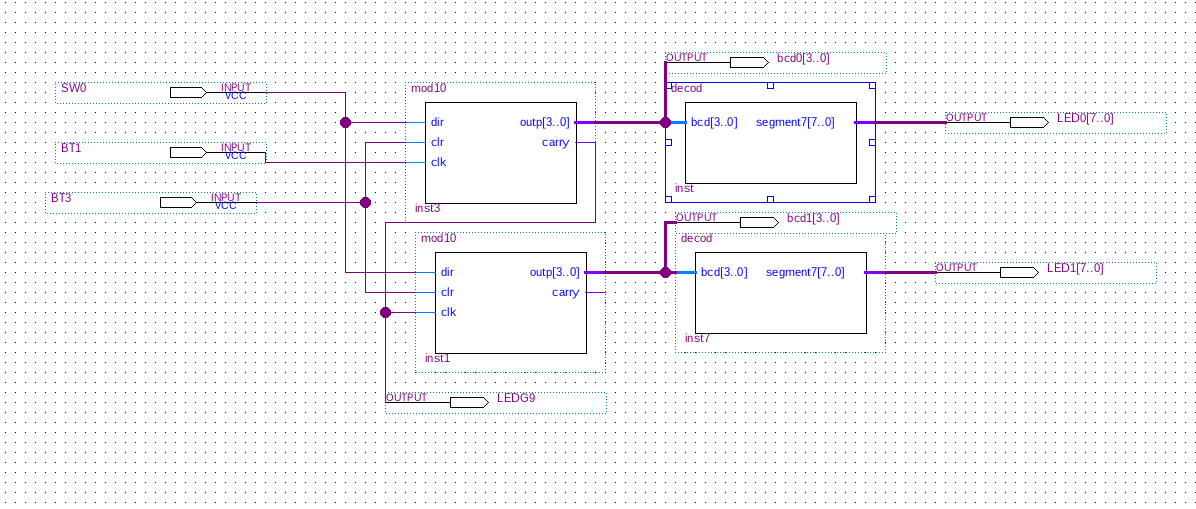
\includegraphics[width=1.0\linewidth]{blok}  % zalacza grafike z rozciagnieciem na cala linie  
	\caption{ Schemat blokowy licznika dla pierwszego wariantu. }
	\label{fig:block_bcd_segment}
\end{figure}


\lstinputlisting[label=lst_mod10,caption=Rewersyjny licznik modulo 10 ,language=VHDL]{mod10.vhd}


\lstinputlisting[label=lst_bcd,caption=Dekoder bcd na 7 segment ,language=VHDL]{decod.vhd}


\subsection{Przebiegi czasowe układu:}
Na rysunkach \ref{fig:symhex0}, \ref{fig:symhex1}, \ref{fig:symhex2}, \ref{fig:symhex3} zostały przedstawione przebiegi czasowe potwierdzające poprawne działanie
licznika rewersyjnego dla pierwszego wariantu. Przycisk BT1 generuje kolejne impulsy zliczające,
natomiast przełącznik suwakowy SW1 steruje kierunkiem zliczanych impulsów (góra, dół).


\begin{figure}[H]
	\centering
	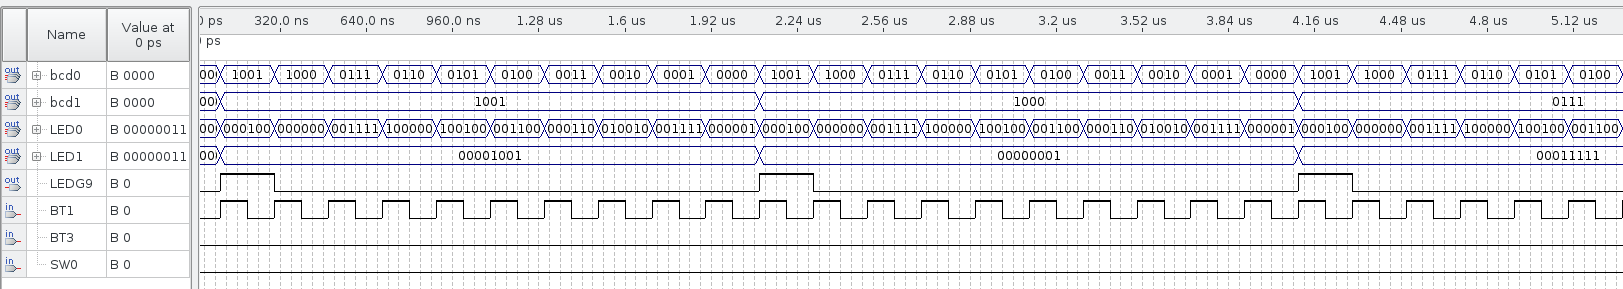
\includegraphics[width=1.0\linewidth]{up_down_1}
	\caption{Przebiegi czasowe – zliczanie w dół (SW0=0)}
	\label{fig:symhex0}
\end{figure}



\begin{figure}[H]
	\centering
	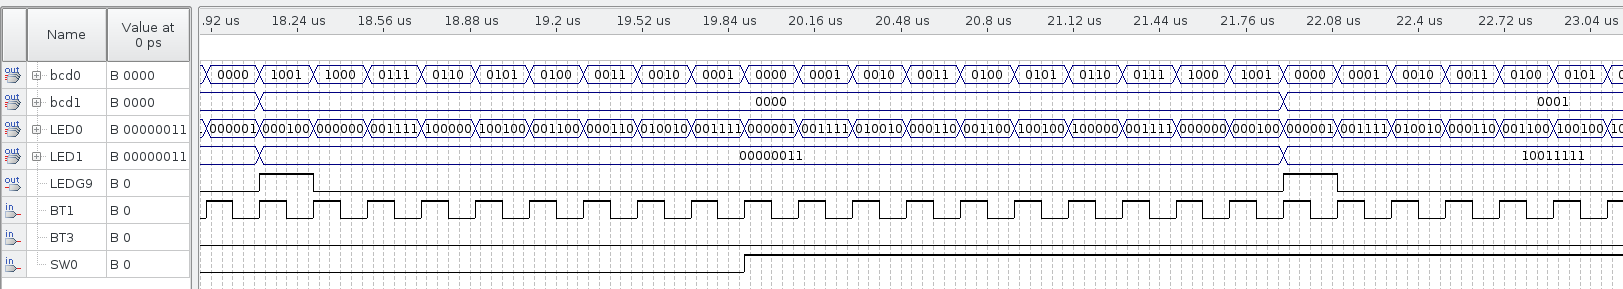
\includegraphics[width=1.0\linewidth]{up_down_2}
	\caption{Przebiegi czasowe – zliczanie w dół (SW0=0 $\longrightarrow$ SW0=1) zmiana pozycji przełącznika suwakowego SW0 przy skrajnych wartościach	}
	\label{fig:symhex1}
\end{figure}



\begin{figure}[H]

S	\centering
	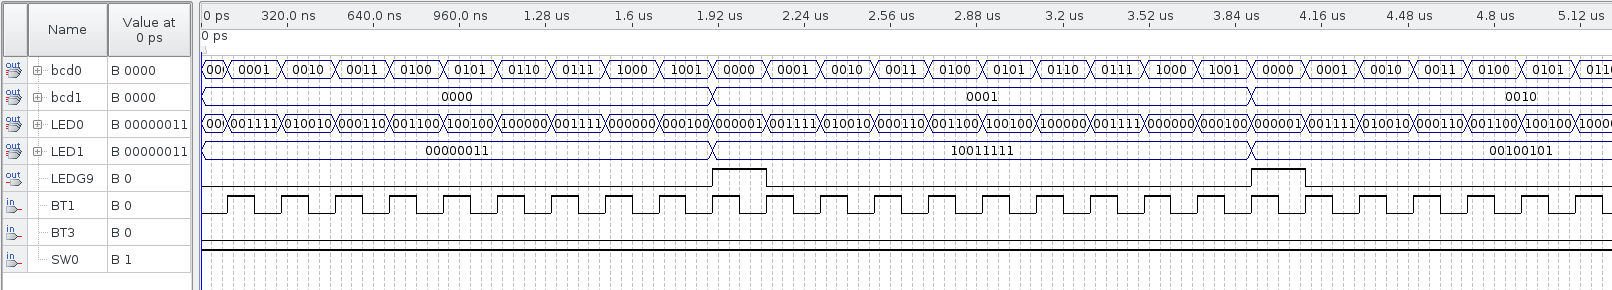
\includegraphics[width=1.0\linewidth]{up_down_inv_1}
	\caption{Przebiegi czasowe – zliczanie w górę (SW0=1) }
	\label{fig:symhex2}
\end{figure}


\begin{figure}[H]
	\centering
	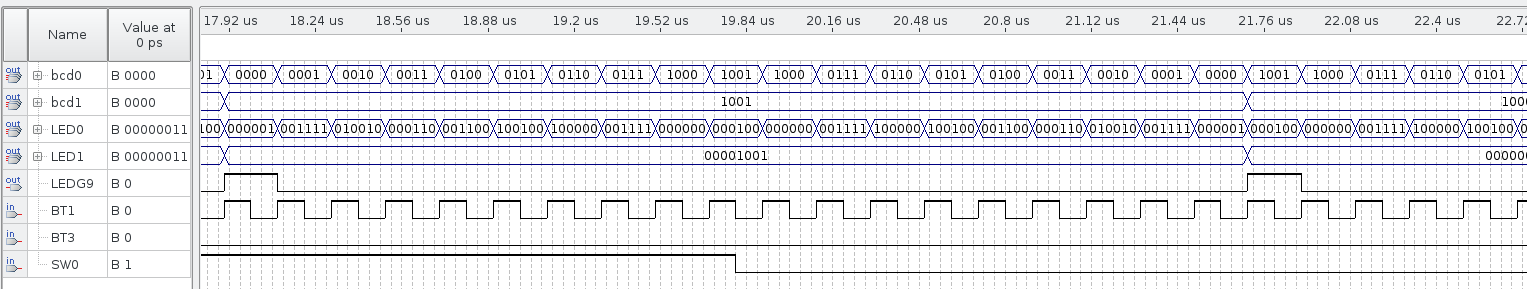
\includegraphics[width=1.0\linewidth]{up_down_inv_2}
	\caption{Przebiegi czasowe – zliczanie w górę (SW0=1 $\longrightarrow$ SW0=0) zmiana pozycji przełącznika suwakowego SW0 przy skrajnych wartościach }
	\label{fig:symhex3}
\end{figure}

\section{ Drugi wariant realizacji projektu licznika}

Realizacja drugiego wariantu polegała na połączeniu dwóch liczników modulo 10 do zliczania
impulsów jedności i dziesiątek, odpowiednie przypisanie wejśd liczników skutkuje odpowiednio
zwiększaniem się liczb na wyświetlaczu po wciśnięciu przycisku BUTTON1, natomiast zmniejszaniu się
wartości po wciśnięciu przycisku BUTTON0.

\begin{figure}[H]  % H - obraz dokladnie w tym miejscu, t - u gory etc..
	\centering
	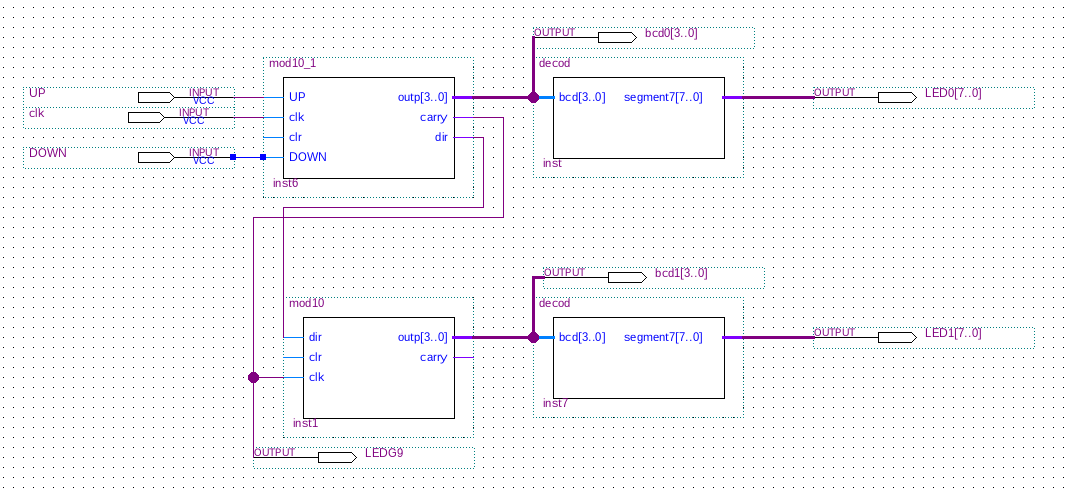
\includegraphics[width=1.0\linewidth]{blok1}  % zalacza grafike z rozciagnieciem na cala linie  
	\caption{ Schemat blokowy licznika dla drugiego wariantu. }
	\label{fig:block1}
\end{figure}

\lstinputlisting[label=lst_mod10_1,caption=Rewersyjny licznik modulo 10 ,language=VHDL]{mod10_1.vhd}

\begin{figure}[H]
	\centering
	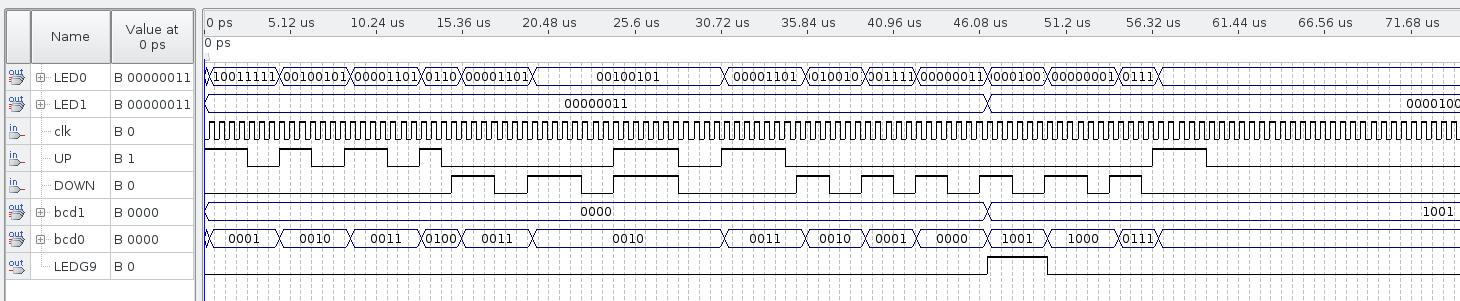
\includegraphics[width=1.0\linewidth]{up_down_1_2}
	\caption{Przebiegi czasowe – zliczanie w dół (SW0=0)}
	\label{fig:symhex0}
\end{figure}

\section{Wnioski}

Celem wykonywanego dwiczenia było zapoznanie się z zasadą działania licznika, oraz jego budową
koniecznymi do realizacji dwóch wariantów licznika rewersyjnego w oprogramowaniu Quartus II. Przy
wykorzystaniu języka VHDL utworzyliśmy nowy bloczek w postaci licznika modulo 10, odpowiednie
połączenie dwóch takich elementów współpracującymi z dekoderami z poprzedniego projektu w
efekcie umożliwiało zaobserwowanie poprawnego działania licznika rewersyjnego.

Odpowiedni amodyfikacja schematu blokowego wraz z kilkoma zmianami w kodzie VHDL umożliwiała realizację
pierwszego wariantu. Utworzony projekt poddawaliśmy testom na poprawnośd działania,
przeprowadzone symulacje są potwierdzeniem założeo projektowych. Ze względu na ograniczony
czas przeznaczony na realizację projektu nie udało się zrealizowad drugiego wariantu, natomiast w
wyniku analizy założeo w sprawozdaniu umieszczono możliwe sposoby realizacji pozwalających
sfinalizowad założenia drugiej opcji.



\begin{thebibliography}{0}
  \bibitem{l2short} John Wiley and Sons Publishers.
    \textsl{Digital Design,} University of California, Riverside, 2007
\end{thebibliography}
\end{document}
